\documentclass[12pt]{article}
\usepackage[paper=letterpaper,margin=2cm]{geometry}
\usepackage{amsmath,amssymb,amsfonts}
\usepackage{newtxtext,newtxmath}
\usepackage{enumitem}
\usepackage{subfig,graphicx}
\usepackage[colorlinks=true]{hyperref}
\usepackage{multirow}
\usepackage{listings}
\usepackage[dvipsnames]{xcolor}
\usepackage{float}
\usepackage[font=small]{caption}

\newcommand{\ind}{\perp\!\!\!\perp}

\definecolor{codegreen}{rgb}{0,0.6,0}
\definecolor{codegray}{rgb}{0.5,0.5,0.5}
\definecolor{codepurple}{rgb}{0.58,0,0.82}
\definecolor{stepscolor}{HTML}{444444}

% BACKGROUND BOX COLORS
\definecolor{byellow}{HTML}{e0b400}
\definecolor{bmint}{HTML}{00c49a}

% \highlight[<colour>]{<stuff>}
\newcommand{\highlight}[2][yellow]{\mathchoice
  {\colorbox{#1}{$\displaystyle#2$}}
  {\colorbox{#1}{$\textstyle#2$}}
  {\colorbox{#1}{$\scriptstyle#2$}}
  {\colorbox{#1}{$\scriptscriptstyle#2$}}}

\lstdefinestyle{mystyle}{
    commentstyle=\color{codegreen},
    keywordstyle=\color{magenta},
    numberstyle=\tiny\color{codegray},
    stringstyle=\color{codepurple},
    basicstyle=\ttfamily\footnotesize,
    breakatwhitespace=false,
    breaklines=true,
    captionpos=b,
    keepspaces=true,
    numbers=left,
    numbersep=6pt,
    showspaces=false,
    showstringspaces=false,
    showtabs=false,
    tabsize=2
}
\lstset{style=mystyle}

\begin{document}
\begin{center}
  \large{Aprendizagem 2023} \\
  Homework IV -- Group 28 \\
  \vskip 0.3cm
  Gonçalo Bárias (ist1103124) \& Raquel Braunschweig (ist1102624)\vskip 1cm

  \large{\textbf{Part I}: Pen and Paper}\normalsize
\end{center}

\noindent Given the following observations, $\left\{\begin{pmatrix} 1 \\ 0.6 \\ 0.1 \end{pmatrix}, \begin{pmatrix} 0 \\ -0.4 \\ 0.8 \end{pmatrix}, \begin{pmatrix} 0 \\ 0.2 \\ 0.5 \end{pmatrix},
  \begin{pmatrix} 1 \\ 0.4 \\ -0.1 \end{pmatrix}\right\}$.

\vskip 0.2cm
\noindent Consider a Bayesian clustering that assumes $\{y_1\} \ind \{y_2, y_3\}$, two clusters following a Bernoulli distribution on $y_1$ ($p_1$ and $p_2$), a multivariate Gaussian on $\{y_2, y_3\}$ ($N_1$ and $N_2$),
and the following initial mixture:

\vskip -0.3cm
\begin{equation*}
  \pi_1 = 0.5 \quad , \quad \pi_2 = 0.5
\end{equation*}
\begin{equation*}
  p_1 = P(y_1 = 1) = 0.3 \quad , \quad p_2 = P(y_1 = 1) = 0.7
\end{equation*}
\begin{equation*}
  \mathcal{N}_1 \left(\boldsymbol{\mu}_1 = \begin{pmatrix} 1 \\ 1 \end{pmatrix}, \mathbf{\Sigma}_1 = \begin{pmatrix} 2 & 0.5 \\ 0.5 & 2 \end{pmatrix}\right) \quad
  , \quad \mathcal{N}_2 \left(\boldsymbol{\mu}_2 = \begin{pmatrix} 0 \\ 0 \end{pmatrix}, \mathbf{\Sigma}_2 = \begin{pmatrix} 1.5 & 1 \\ 1 & 1.5 \end{pmatrix}\right)
\end{equation*}

\vskip 0.2cm
\begin{enumerate}[leftmargin=\labelsep]
  \item \textbf{Perform one epoch of the EM clustering algorithm and determine the new parameters.}\\
        \textbf{\textit{Hint:} we suggest you to use numpy and scipy, however disclose the intermediary results step by step.}

        \vskip 0.3cm
        The EM (Expectation-Maximization) algorithm has four major steps: Initialization, Expectation, Maximization and Verification.

        \vskip 0.2cm
          {
            \color{stepscolor}
            \begin{large}\textbf{1. Initialization}\end{large}
          }
        \vskip 0.1cm

        We'll start by labeling each observation:

        $$
          x_1 = \begin{pmatrix} 1 \\ 0.6 \\ 0.1 \end{pmatrix}
          \quad,\quad
          x_2 = \begin{pmatrix} 0 \\ -0.4 \\ 0.8 \end{pmatrix}
          \quad,\quad
          x_3 = \begin{pmatrix} 0 \\ 0.2 \\ 0.5 \end{pmatrix}
          \quad,\quad
          x_4 = \begin{pmatrix} 1 \\ 0.4 \\ -0.1 \end{pmatrix}
        $$

        From the statement we have the following initial parameters, $p_1$, $p_2$, $\mu_1$, $\mu_2$, $\Sigma_1$,
        $\Sigma_2$, $\pi_1$ and $\pi_2$:

        \begin{center}
          \captionsetup{type=table}
          \begin{tabular}{c|cccc}
            Cluster                                            & $p$ & $\mu$ & $\Sigma$ & $\pi$ \\
            \hline
            \colorbox{bmint}{Cluster 1}                        &
            0.3                                                &
            $\begin{pmatrix} 1 \\ 1 \end{pmatrix}$             &
            $\begin{pmatrix} 2 & 0.5 \\ 0.5 & 2 \end{pmatrix}$ &
            0.5                                                                                 \\
            \colorbox{byellow}{Cluster 2}                      &
            0.7                                                &
            $\begin{pmatrix} 0 \\ 0 \end{pmatrix}$             &
            $\begin{pmatrix} 1.5 & 1 \\ 1 & 1.5 \end{pmatrix}$ &
            0.5                                                                                 \\
          \end{tabular}
          \captionof{table}{Initial parameters for the two clusters}
          \label{exI1-initial-params-table}
        \end{center}

        \vskip 0.2cm
          {
            \color{stepscolor}
            \begin{large}\textbf{2. Expectation (E-step)}\end{large}
          }
        \vskip 0.1cm

        Considering $\{y_1\} \ind \{y_2, y_3\}$ we know the posterior probability, $P(c_k | x_i)$, is given by Baye's rule:

        \begin{equation}\label{exI1-posterior}
          P(c_k | x_i) = \frac{P(y_1,y_2,y_3|c_k)P(c_k)}{P(y_1,y_2,y_3)} = \frac{P(y_1|c_k)P(y_2,y_3|c_k)P(c_k)}{P(y_1)P(y_2,y_3)}
        \end{equation}

        Since we know that $\sum_j P(c_j|x_i)$ must be equal to 1, we need to normalize the values given by equation \eqref{exI1-posterior}.
        Therefore, we get these new normalized values for the posteriors represented by $\gamma_{k,i}$:

        \begin{equation}\label{exI1-gamma}
          \gamma_{k,i} = \frac{P(c_k | x_i)}{\sum_j P(c_j | x_i)}
          = \frac{P(y_1|c_k)P(y_2,y_3|c_k)P(c_k)}{\sum_j P(y_1|c_j)P(y_2,y_3|c_j)P(c_j)}
        \end{equation}

        The variable $y_1$ follows a Bernoulli distribution ($y_1 \sim \text{Bern}\left(p=p_k\right)$), and so the likelihoods,\\
        $P(y_1=0|c_k)$ and $P(y_1=1|c_k)$, can be calculated for each cluster:

        \vskip -0.4cm
        \begin{align*}
          P(y_1 = 0 | c_1) = 1 - p_1 = 1 - 0.3 = 0.7 & \qquad P(y_1 = 0 | c_2) = 1 - p_2 = 1 - 0.7 = 0.3 \\
          P(y_1 = 1 | c_1) = p_1 = 0.3               & \qquad P(y_1 = 1 | c_2) = p_2 = 0.7
        \end{align*}

        We know the likelihood, $P(y_2,y_3|c_k)$, follows a multivariate Gaussian, and so it is given by
        (considering $d = 2$, since we are working in two dimensions):

        \vskip -0.2cm
        \begin{equation}\label{exI1-likelihood-multivariate}
          P(y_2=a,y_3=b|c_k) = \mathcal{N}_k(y_2=a,y_3=b|\mu_k, \Sigma_k)
          = \frac{
          \exp\left(-\frac{1}{2} \left(\begin{bmatrix} a \\ b \end{bmatrix} - \mu_k\right)^T
          \Sigma_k^{-1} \left(\begin{bmatrix} a \\ b \end{bmatrix} - \mu_k\right)\right)}{(2\pi)^{d/2} \times |\Sigma_k|^{1/2}}
        \end{equation}

        We now have all the building blocks to calculate the posterior probabilities
        for each combination of observation, $x_i$ and cluster, $c_k$.

        We'll start off by calculating the multivariate likelihood by employing equation
        \eqref{exI1-likelihood-multivariate}, for each pair of observation and cluster:

        \begin{center}
          \textbf{\colorbox{bmint}{Cluster 1 Multivariate Likelihoods}}
        \end{center}

        \vskip -0.7cm
        \begingroup
        \addtolength{\jot}{0.5em}
        \begin{align*}
          P(y_2=0.6, y_3=0.1 | c_1)  & = \mathcal{N}_1(y_2=0.6, y_3=0.1|\mu_1, \Sigma_1) \approx 0.06658  \\
          P(y_2=-0.4, y_3=0.8 | c_1) & = \mathcal{N}_1(y_2=-0.4, y_3=0.8|\mu_1, \Sigma_1) \approx 0.05005 \\
          P(y_2=0.2, y_3=0.5 | c_1)  & = \mathcal{N}_1(y_2=0.2, y_3=0.5|\mu_1, \Sigma_1) \approx 0.06837  \\
          P(y_2=0.4, y_3=-0.1 | c_1) & = \mathcal{N}_1(y_2=0.4, y_3=-0.1|\mu_1, \Sigma_1) \approx 0.05905
        \end{align*}
        \endgroup

        \begin{center}
          \textbf{\colorbox{byellow}{Cluster 2 Multivariate Likelihood}}
        \end{center}

        \vskip -0.7cm
        \begingroup
        \addtolength{\jot}{0.7em}
        \begin{align*}
          P(y_2=0.6, y_3=0.1 | c_2)  & = \mathcal{N}_2(y_2=0.6, y_3=0.1|\mu_2, \Sigma_2) \approx 0.11962  \\
          P(y_2=-0.4, y_3=0.8 | c_2) & = \mathcal{N}_2(y_2=-0.4, y_3=0.8|\mu_2, \Sigma_2) \approx 0.06819 \\
          P(y_2=0.2, y_3=0.5 | c_2)  & = \mathcal{N}_2(y_2=0.2, y_3=0.5|\mu_2, \Sigma_2) \approx 0.12958  \\
          P(y_2=0.4, y_3=-0.1 | c_2) & = \mathcal{N}_2(y_2=0.4, y_3=-0.1|\mu_2, \Sigma_2) \approx 0.12450
        \end{align*}
        \endgroup

        \vskip 0.1cm
        Finally, we can employ equation \eqref{exI1-gamma} to calculate the normalized posteriors with the previously calculated values,
        for each pair of observation and cluster:

        \begin{center}
          \textbf{\colorbox{bmint}{Cluster 1 Posteriors}}
        \end{center}

        \vskip -0.5cm
        \begingroup
        \addtolength{\jot}{0.7em}
        \begin{align*}
          \gamma_{1,1} & = \frac{P(y_1=1|c_1)P(y_2=0.6,y_3=0.1|c_1)P(c_1)}{P(y_1=1|c_1)P(y_2=0.6,y_3=0.1|c_1)P(c_1) + P(y_1=1|c_2)P(y_2=0.6,y_3=0.1|c_2)P(c_2)}    \\
                       & = \frac{0.3 \times 0.06658 \times 0.5}{0.3 \times 0.06658 \times 0.5 + 0.7 \times 0.11962 \times 0.5} \approx 0.19259                     \\
          \gamma_{1,2} & = \frac{P(y_1=0|c_1)P(y_2=-0.4,y_3=0.8|c_1)P(c_1)}{P(y_1=0|c_1)P(y_2=-0.4,y_3=0.8|c_1)P(c_1) + P(y_1=0|c_2)P(y_2=-0.4,y_3=0.8|c_2)P(c_2)} \\
                       & = \frac{0.7 \times 0.05005 \times 0.5}{0.7 \times 0.05005 \times 0.5 + 0.3 \times 0.06819 \times 0.5} \approx 0.63135                     \\
          \gamma_{1,3} & = \frac{P(y_1=0|c_1)P(y_2=0.2,y_3=0.5|c_1)P(c_1)}{P(y_1=0|c_1)P(y_2=0.2,y_3=0.5|c_1)P(c_1) + P(y_1=0|c_2)P(y_2=0.2,y_3=0.5|c_2)P(c_2)}    \\
                       & = \frac{0.7 \times 0.06837 \times 0.5}{0.7 \times 0.06837 \times 0.5 + 0.3 \times 0.12958 \times 0.5} \approx 0.55181                     \\
          \gamma_{1,4} & = \frac{P(y_1=1|c_1)P(y_2=0.4,y_3=-0.1|c_1)P(c_1)}{P(y_1=1|c_1)P(y_2=0.4,y_3=-0.1|c_1)P(c_1) + P(y_1=1|c_2)P(y_2=0.4,y_3=-0.1|c_2)P(c_2)} \\
                       & = \frac{0.3 \times 0.05905 \times 0.5}{0.3 \times 0.05905 \times 0.5 + 0.7 \times 0.12450 \times 0.5} \approx 0.16892
        \end{align*}
        \endgroup

        \begin{center}
          \textbf{\colorbox{byellow}{Cluster 2 Posteriors}}
        \end{center}

        \vskip -0.5cm
        \begingroup
        \addtolength{\jot}{0.5em}
        \begin{align*}
          \gamma_{2,1} & = \frac{P(y_1=1|c_2)P(y_2=0.6,y_3=0.1|c_2)P(c_2)}{P(y_1=1|c_1)P(y_2=0.6,y_3=0.1|c_1)P(c_1) + P(y_1=1|c_2)P(y_2=0.6,y_3=0.1|c_2)P(c_2)}    \\
                       & = \frac{0.7 \times 0.11962 \times 0.5}{0.3 \times 0.06658 \times 0.5 + 0.7 \times 0.11962 \times 0.5} \approx 0.80741                     \\
          \gamma_{2,2} & = \frac{P(y_1=0|c_2)P(y_2=-0.4,y_3=0.8|c_2)P(c_2)}{P(y_1=0|c_1)P(y_2=-0.4,y_3=0.8|c_1)P(c_1) + P(y_1=0|c_2)P(y_2=-0.4,y_3=0.8|c_2)P(c_2)} \\
                       & = \frac{0.3 \times 0.06819 \times 0.5}{0.7 \times 0.05005 \times 0.5 + 0.3 \times 0.06819 \times 0.5} \approx 0.36865                     \\
          \gamma_{2,3} & = \frac{P(y_1=0|c_2)P(y_2=0.2,y_3=0.5|c_2)P(c_2)}{P(y_1=0|c_1)P(y_2=0.2,y_3=0.5|c_1)P(c_1) + P(y_1=0|c_2)P(y_2=0.2,y_3=0.5|c_2)P(c_2)}    \\
                       & = \frac{0.3 \times 0.12958 \times 0.5}{0.7 \times 0.06837 \times 0.5 + 0.3 \times 0.12958 \times 0.5} \approx 0.44819                     \\
          \gamma_{2,4} & = \frac{P(y_1=1|c_2)P(y_2=0.4,y_3=-0.1|c_2)P(c_2)}{P(y_1=1|c_1)P(y_2=0.4,y_3=-0.1|c_1)P(c_1) + P(y_1=1|c_2)P(y_2=0.4,y_3=-0.1|c_2)P(c_2)} \\
                       & = \frac{0.7 \times 0.12450 \times 0.5}{0.3 \times 0.05905 \times 0.5 + 0.7 \times 0.12450 \times 0.5} \approx 0.83108
        \end{align*}
        \endgroup

        \vskip 0.2cm
          {
            \color{stepscolor}
            \begin{large}\textbf{3. Maximization (M-step)}\end{large}
          }
        \vskip 0.1cm

        Below we will use ${x_i}_{[y_1]}$ to refer to the variable $\{y_1\}$ of observation $x_i$ and
        ${x_i}_{[y_2 \land y_3]}$ to refer to the variables $\{y_2,y_3\}$ of observation $x_i$.

        For each cluster, $c_k$, we will calculate the following in order to update the parameters:

        \begin{equation}\label{exI1-Nk}
          N_k = \sum_i \gamma_{k,i}
        \end{equation}
        \begin{equation}\label{exI1-pk}
          p_k' = \frac{1}{N_k} \sum_{i} \gamma_{k,i} \cdot {x_i}_{[y_1]}
        \end{equation}
        \begin{equation}\label{exI1-muk}
          \mu_k' = \frac{1}{N_k} \sum_{i} \gamma_{k,i} \cdot {x_i}_{[y_2 \land y_3]}
        \end{equation}
        \begin{equation}\label{exI1-sigmak}
          \Sigma_k' = \frac{1}{N_k} \sum_{i} \gamma_{k,i} \cdot \left({x_i}_{[y_2 \land y_3]} - \mu_k'\right) \cdot ({x_i}_{[y_2 \land y_3]} - \mu_k')^T
        \end{equation}

        Considering $N = \sum_k N_k$, we can also update the priors:

        \begin{equation}\label{exI1-pik}
          \pi_k' = \frac{N_k}{N}
        \end{equation}

        We can now update the values for both clusters using the previous equations.

        We start off by calculating the sum of the weights, for each cluster, $N_k$, by employing equation \eqref{exI1-Nk}:

        \begin{equation*}
          \highlight[bmint]{N_1} = \sum_{i} \gamma_{1,i} = \gamma_{1,1} + \gamma_{1,2} + \gamma_{1,3} + \gamma_{1,4} = 1.54467
        \end{equation*}
        \begin{equation*}
          \highlight[byellow]{N_2} = \sum_{i} \gamma_{2,i} = \gamma_{2,1} + \gamma_{2,2} + \gamma_{2,3} + \gamma_{2,4} = 2.45533
        \end{equation*}

        \begin{center}
          \textbf{\colorbox{bmint}{Cluster 1 Updates}}
        \end{center}

        Now for cluster 1 we can update $p_1$, $\mu_1$, $\Sigma_1$ and $\pi_1$, by employing, \eqref{exI1-pk}, \eqref{exI1-muk},
        \eqref{exI1-sigmak} and \eqref{exI1-pik}, respectively:

        \begingroup
        \allowdisplaybreaks
        \begin{equation*}
          p_1' = \frac{1}{N_1} \sum_{i} \gamma_{1,i} \cdot {x_i}_{[y_1]}
          = \frac{\gamma_{1,1} \cdot 1
            + \gamma_{1,2} \cdot 0
            + \gamma_{1,3} \cdot 0
            + \gamma_{1,4} \cdot 1}{1.54467}
          = 0.23404
        \end{equation*}
        \endgroup

        \begingroup
        \allowdisplaybreaks
        \begin{equation*}
          \mu_1' = \frac{1}{N_1} \sum_{i} \gamma_{1,i} \cdot {x_i}_{[y_2 \land y_3]}
          = \frac{\gamma_{1,1} \cdot \begin{pmatrix} 0.6 \\ 0.1 \end{pmatrix}
            + \gamma_{1,2} \cdot \begin{pmatrix} -0.4 \\ 0.8 \end{pmatrix}
            + \gamma_{1,3} \cdot \begin{pmatrix} 0.2 \\ 0.5 \end{pmatrix}
            + \gamma_{1,4} \cdot \begin{pmatrix} 0.4 \\ -0.1 \end{pmatrix}}{1.54467}
          = \begin{pmatrix} 0.02651 \\ 0.50713 \end{pmatrix}
        \end{equation*}
        \endgroup

        \begingroup
        \allowdisplaybreaks
        \begin{align*}
          \Sigma_1' & = \frac{1}{N_1} \sum_{i} \gamma_{1,i} \cdot \left({x_i}_{[y_2 \land y_3]} - \mu_1'\right) \cdot ({x_i}_{[y_2 \land y_3]} - \mu_1')^T                                                                                                             \\
                    & = \frac{1}{1.54467} \times \Bigg[ \Bigg.
          \gamma_{1,1} \cdot \left(\begin{pmatrix} 0.6 \\ 0.1 \end{pmatrix} - \begin{pmatrix} 0.02651 \\ 0.50713 \end{pmatrix}\right) \cdot \left(\begin{pmatrix} 0.6 \\ 0.1 \end{pmatrix} - \begin{pmatrix} 0.02651 \\ 0.50713 \end{pmatrix}\right)^T                 \\
                    & + \gamma_{1,2} \cdot \left(\begin{pmatrix} -0.4 \\ 0.8 \end{pmatrix} - \begin{pmatrix} 0.02651 \\ 0.50713 \end{pmatrix}\right) \cdot \left(\begin{pmatrix} -0.4 \\ 0.8 \end{pmatrix} - \begin{pmatrix} 0.02651 \\ 0.50713 \end{pmatrix}\right)^T \\
                    & + \gamma_{1,3} \cdot \left(\begin{pmatrix} 0.2 \\ 0.5 \end{pmatrix} - \begin{pmatrix} 0.02651 \\ 0.50713 \end{pmatrix}\right) \cdot \left(\begin{pmatrix} 0.2 \\ 0.5 \end{pmatrix} - \begin{pmatrix} 0.02651 \\ 0.50713 \end{pmatrix}\right)^T   \\
                    & + \gamma_{1,4} \cdot \left(\begin{pmatrix} 0.4 \\ -0.1 \end{pmatrix} - \begin{pmatrix} 0.02651 \\ 0.50713 \end{pmatrix}\right) \cdot \left(\begin{pmatrix} 0.4 \\ -0.1 \end{pmatrix} - \begin{pmatrix} 0.02651 \\ 0.50713 \end{pmatrix}\right)^T
          \Bigg. \Bigg]                                                                                                                                                                                                                                                \\
                    & = \begin{pmatrix} 0.14137 & -0.10541 \\ -0.10541 & 0.09605 \end{pmatrix}
        \end{align*}
        \endgroup

        \begin{equation*}
          \pi_1' = \frac{N_1}{N} = \frac{N_1}{N_1 + N_2} = \frac{1.54467}{1.54467 + 2.45533} = 0.38617
        \end{equation*}

        \begin{center}
          \textbf{\colorbox{byellow}{Cluster 2 Updates}}
        \end{center}

        Finally, for cluster 2 we can update $p_2$, $\mu_2$, $\Sigma_2$ and $\pi_2$, by employing, \eqref{exI1-pk}, \eqref{exI1-muk},
        \eqref{exI1-sigmak} and \eqref{exI1-pik}, respectively:

        \begingroup
        \allowdisplaybreaks
        \begin{equation*}
          p_2' = \frac{1}{N_2} \sum_{i} \gamma_{2,i} \cdot {x_i}_{[y_1]}
          = \frac{\gamma_{2,1} \cdot 1
            + \gamma_{2,2} \cdot 0
            + \gamma_{2,3} \cdot 0
            + \gamma_{2,4} \cdot 1}{2.45533}
          = 0.66732
        \end{equation*}
        \endgroup

        \begingroup
        \allowdisplaybreaks
        \begin{equation*}
          \mu_2' = \frac{1}{N_2} \sum_{i} \gamma_{2,i} \cdot {x_i}_{[y_2 \land y_3]}
          = \frac{\gamma_{2,1} \cdot \begin{pmatrix} 0.6 \\ 0.1 \end{pmatrix}
            + \gamma_{2,2} \cdot \begin{pmatrix} -0.4 \\ 0.8 \end{pmatrix}
            + \gamma_{2,3} \cdot \begin{pmatrix} 0.2 \\ 0.5 \end{pmatrix}
            + \gamma_{2,4} \cdot \begin{pmatrix} 0.4 \\ -0.1 \end{pmatrix}}{2.45533}
          = \begin{pmatrix} 0.30914 \\ 0.21042 \end{pmatrix}
        \end{equation*}
        \endgroup

        \begingroup
        \allowdisplaybreaks
        \begin{align*}
          \Sigma_2' & = \frac{1}{N_2} \sum_{i} \gamma_{2,i} \cdot \left({x_i}_{[y_2 \land y_3]} - \mu_2'\right) \cdot ({x_i}_{[y_2 \land y_3]} - \mu_2')^T                                                                                                             \\
                    & = \frac{1}{2.45533} \times \Bigg[ \Bigg.
          \gamma_{2,1} \cdot \left(\begin{pmatrix} 0.6 \\ 0.1 \end{pmatrix} - \begin{pmatrix} 0.30914 \\ 0.21042 \end{pmatrix}\right) \cdot \left(\begin{pmatrix} 0.6 \\ 0.1 \end{pmatrix} - \begin{pmatrix} 0.30914 \\ 0.21042 \end{pmatrix}\right)^T                 \\
                    & + \gamma_{2,2} \cdot \left(\begin{pmatrix} -0.4 \\ 0.8 \end{pmatrix} - \begin{pmatrix} 0.30914 \\ 0.21042 \end{pmatrix}\right) \cdot \left(\begin{pmatrix} -0.4 \\ 0.8 \end{pmatrix} - \begin{pmatrix} 0.30914 \\ 0.21042 \end{pmatrix}\right)^T \\
                    & + \gamma_{2,3} \cdot \left(\begin{pmatrix} 0.2 \\ 0.5 \end{pmatrix} - \begin{pmatrix} 0.30914 \\ 0.21042 \end{pmatrix}\right) \cdot \left(\begin{pmatrix} 0.2 \\ 0.5 \end{pmatrix} - \begin{pmatrix} 0.30914 \\ 0.21042 \end{pmatrix}\right)^T   \\
                    & + \gamma_{2,4} \cdot \left(\begin{pmatrix} 0.4 \\ -0.1 \end{pmatrix} - \begin{pmatrix} 0.30914 \\ 0.21042 \end{pmatrix}\right) \cdot \left(\begin{pmatrix} 0.4 \\ -0.1 \end{pmatrix} - \begin{pmatrix} 0.30914 \\ 0.21042 \end{pmatrix}\right)^T
          \Bigg. \Bigg]                                                                                                                                                                                                                                                \\
                    & = \begin{pmatrix} 0.10829 & -0.08865 \\ -0.08865 & 0.10412 \end{pmatrix}
        \end{align*}
        \endgroup

        \begin{equation*}
          \pi_2' = \frac{N_2}{N} = \frac{N_2}{N_1 + N_2} = \frac{2.45533}{1.54467 + 2.45533} = 0.61383
        \end{equation*}

        \vskip 0.2cm
          {
            \color{stepscolor}
            \begin{large}\textbf{4. Verify the log likelihood}\end{large}
            \vskip 0.1cm
          }

        Since we are only performing one epoch of the EM clustering algorithm, we can skip this step.

        \vskip 0.2cm
          {
            \color{stepscolor}
            \begin{large}\textbf{5. Conclusion}\end{large}
            \vskip 0.1cm
          }

        After performing one epoch of the EM clustering algorithm, we end up with the following updated parameters for each cluster:

        \begin{center}
          \captionsetup{type=table}
          \begin{tabular}{c|cccc}
            Cluster                                                                  & $p'$ & $\mu'$ & $\Sigma'$ & $\pi'$ \\
            \hline
            \colorbox{bmint}{Cluster 1}                                              &
            0.23404                                                                  &
            $\begin{pmatrix} 0.02651 \\ 0.50713 \end{pmatrix}$                       &
            $\begin{pmatrix} 0.14137 & -0.10541 \\ -0.10541 & 0.09605 \end{pmatrix}$ &
            0.38617                                                                                                       \\
            \colorbox{byellow}{Cluster 2}                                            &
            0.66732                                                                  &
            $\begin{pmatrix} 0.30914 \\ 0.21042 \end{pmatrix}$                       &
            $\begin{pmatrix} 0.10829 & -0.08865 \\ -0.08865 & 0.10412 \end{pmatrix}$ &
            0.61383                                                                                                       \\
          \end{tabular}
          \captionof{table}{Updated parameters for the two clusters after one epoch of the EM clustering algorithm}
          \label{exI1-updated-params-table}
        \end{center}

  \item \textbf{Given the new observation, $x_{new} = \begin{bmatrix} 1 & 0.3 & 0.7 \end{bmatrix}^T$, determine the cluster memberships (posteriors).}

        \vskip 0.3cm
        \textbf{Note:} As per the \textit{FAQ}, we will be using the updated values obtained in exercise 1.

        Using the equation on \eqref{exI1-likelihood-multivariate}, we can compute, for each cluster, $c_k$,
        the value of $P(y_2,y_3|c_k)$ for the new observation, $x_{new}$:

        \vskip -0.5cm
        \begingroup
        \addtolength{\jot}{0.7em}
        \begin{align*}
          P(y_2=0.3,y_3=0.7|c_1) = \mathcal{N}_1(y_2=0.3, y_3=0.7 | \mu'_1, \Sigma'_{1}) \approx 0.02708 \\
          P(y_2=0.3,y_3=0.7|c_2) = \mathcal{N}_2(y_2=0.3, y_3=0.7 | \mu'_2, \Sigma'_{2}) \approx 0.06843
        \end{align*}
        \endgroup

        Now, by using the equation on \eqref{exI1-gamma}, we can compute the normalized posteriors:

        \vskip -0.3cm
        \begingroup
        \addtolength{\jot}{0.7em}
        \begin{align*}
          \gamma_{1, new} & = \frac{P(y_1=1|c_1)P(y_2=0.3,y_3=0.7|c_1)P(c_1)}{P(y_1=1|c_1)P(y_2=0.3,y_3=0.7|c_1)P(c_1) + P(y_1=1|c_2)P(y_2=0.3,y_3=0.7|c_2)P(c_2)}        \\
                          & = \frac{p_1' \times 0.02708 \times \pi_1'}{p_1' \times 0.02708 \times \pi_1' + p_2' \times 0.06843 \times \pi_2'}                             \\
                          & = \frac{0.23404 \times 0.02708 \times 0.38617}{0.23404 \times 0.02708 \times 0.38617 + 0.66732 \times 0.06843 \times 0.61383} \approx 0.08029 \\
          \gamma_{2, new} & = \frac{P(y_1=1|c_2)P(y_2=0.3,y_3=0.7|c_2)P(c_2)}{P(y_1=1|c_1)P(y_2=0.3,y_3=0.7|c_1)P(c_1) + P(y_1=1|c_2)P(y_2=0.3,y_3=0.7|c_2)P(c_2)}        \\
                          & = \frac{p_2' \times 0.06843 \times \pi_2'}{p_1' \times 0.02708 \times \pi_1' + p_2' \times 0.06843 \times \pi_2'}                             \\
                          & = \frac{0.66732 \times 0.06843 \times 0.61383}{0.23404 \times 0.02708 \times 0.38617 + 0.66732 \times 0.06843 \times 0.61383} \approx 0.91971
        \end{align*}
        \endgroup

  \item \textbf{Performing a hard assignment of observations to clusters under a ML assumption, identify the silhouette of both clusters under a Manhattan distance.}

        \vskip 0.3cm
        \textbf{Note:} As per the \textit{FAQ}, we will be using the updated values obtained in exercise 1 and only show the calculus for the
        observation $x_2$, only presenting the remaining results in Table \ref{exI3-likelihood-table}.

        Firstly, we need to calculate the updated likelihoods. For that, we consider $\{y_1\} \ind \{y_2, y_3\}$ and multiply $P(y_1|c_k)$ by $P(y_2,y_3|c_k)$,
        which is given by the equation \eqref{exI1-likelihood-multivariate}:

        \vskip -0.4cm
        \begingroup
        \addtolength{\jot}{0.5em}
        \begin{align*}
          P(x_2 | c_1) & = P(y_1 = 0 | c_1) \times P(y_2 = -0.4, y_3 = 0.8 | c_1)
          = (1 - p_1') \times \mathcal{N}_1(y_2 = -0.4, y_3 = 0.8 | \mu_1', \Sigma_1') \\
                       & = 0.76596 \times 1.65326 \approx 1.26633                      \\
          P(x_2 | c_2) & = P(y_1 = 0 | c_2) \times P(y_2 = -0.4, y_3 = 0.8 | c_2)
          = (1 - p_2') \times \mathcal{N}_2(y_2 = -0.4, y_3 = 0.8 | \mu_2', \Sigma_2') \\
                       & = 0.33268 \times 0.26673 \approx 0.08874
        \end{align*}
        \endgroup

        \vskip 0.2cm
        \begin{center}
          \captionsetup{type=table}
          \begin{tabular}{c|cccc}
            Cluster                               & $P(x_1 | c_k)$ & $P(x_2 | c_k)$ & $P(x_3 | c_k)$ & $P(x_4 | c_k)$ \\
            \hline
            \colorbox{bmint}{Cluster 1} ($c_1$)   &
            0.23147                               &
            1.26633                               &
            1.43811                               &
            0.02077                                                                                                   \\
            \colorbox{byellow}{Cluster 2} ($c_2$) &
            0.94954                               &
            0.08874                               &
            0.45417                               &
            0.72331                                                                                                   \\
          \end{tabular}
          \captionof{table}{Updated likelihoods for the two clusters}
          \label{exI3-likelihood-table}
        \end{center}

        Based on the calculated likelihoods, we can infer that $x_1$ and $x_4$ are assigned to Cluster 2, while $x_2$ and $x_3$ are assigned to Cluster 1:

        \vskip -0.3cm
        \begin{equation*}
          C_1 = \{x_2, x_3\} \qquad\qquad C_2 = \{x_1, x_4\}
        \end{equation*}

        The Manhattan distance is given by the following equation:

        \begin{equation}\label{exI3-manhattan}
          d(P, Q) = d((a_1, b_1, c_1), (a_2, b_2, c_2))= |a_2 - a_1| + |b_2 - b_1| + |c_2 - c_1|
        \end{equation}

        By employing equation \eqref{exI3-manhattan}, we can create the Table \ref{exI3-manhattan-distances} that has the manhattan
        distances between every pair of observations. Only the upper diagonal entries are filled, because the distance function is commutative.

        \begin{center}
          \captionsetup{type=table}
          \begin{tabular}{c|cccc}
            $d(x_i, x_j)$ & $x_1$ & $x_2$ & $x_3$ & $x_4$ \\
            \hline
            $x_1$         & 0     & 2.7   & 1.8   & 0.4   \\
            $x_2$         & -     & 0     & 0.9   & 2.7   \\
            $x_3$         & -     & -     & 0     & 1.8   \\
            $x_4$         & -     & -     & -     & 0
          \end{tabular}
          \captionof{table}{Manhattan distances between every pair of observations}
          \label{exI3-manhattan-distances}
        \end{center}

        The Cohesion ($a(x_i)$), Separation ($b(x_i)$) and Silhouette ($S(x_i)$), for a given observation $x_i$, are given by:

        \vskip -0.3cm
        \begin{equation*}
          \begin{aligned}
            a(x_i) & = \text{average distance of} \; x_i \; \text{to the other points in its cluster}                                                    \\
            b(x_i) & = \text{min}_j\{\text{average distance of} \; x_i \; \text{to the points of cluster} \; C_j \; \text{such that} \; x_i \notin C_j\}
          \end{aligned}
        \end{equation*}

        \begin{equation}\label{exI3-silhouette}
          S(x_i) = \frac{b(x_i) - a(x_i)}{\max\{b(x_i), a(x_i)\}}
        \end{equation}

        The silhouette for a cluster $C_k$ is given by:

        \begin{equation}\label{exI3-silhouette-cluster}
          S(C_k) = \frac{\sum_{x_i \in C_k} S(x_i)}{\left|C_k\right|}
        \end{equation}

        By replacing the values on the equation \eqref{exI3-silhouette}, we get the following values:

        \begingroup
        \allowdisplaybreaks
        \addtolength{\jot}{0.7em}
        \begin{align*}
          S(x_1) & = \frac{\frac{d(x_1, x_2) \,+\, d(x_1, x_3)}{2} - d(x_1,x_4)}{\max\left\{\frac{d(x_1, x_2) \,+\, d(x_1, x_3)}{2}, d(x_1,x_4)\right\}}
          = \frac{2.25 - 0.4}{\max\left\{2.25, 0.4\right\}} = \frac{2.25 - 0.4}{2.25} \approx 0.82222                                                    \\
          S(x_2) & = \frac{\frac{d(x_2, x_1) \,+\, d(x_2, x_4)}{2} - d(x_2,x_3)}{\max\left\{\frac{d(x_2, x_1) \,+\, d(x_2, x_4)}{2}, d(x_2,x_3)\right\}}
          = \frac{2.7 - 0.9}{\max\left\{2.7, 0.9\right\}} = \frac{2.7 - 0.9}{2.7} \approx 0.66667                                                        \\
          S(x_3) & = \frac{\frac{d(x_3, x_1) \,+\, d(x_3, x_4)}{2} - d(x_3,x_2)}{\max\left\{\frac{d(x_3, x_1) \,+\, d(x_3, x_4)}{2}, d(x_3,x_2)\right\}}
          = \frac{1.8 - 0.9}{\max\left\{1.8, 0.9\right\}} = \frac{1.8 - 0.9}{1.8} = 0.5                                                                  \\
          S(x_4) & = \frac{\frac{d(x_4, x_2) \,+\, d(x_4, x_3)}{2} - d(x_4,x_1)}{\max\left\{\frac{d(x_4, x_2) \,+\, d(x_4, x_3)}{2}, d(x_4,x_1)\right\}}
          = \frac{2.25 - 0.4}{\max\left\{2.25, 0.4\right\}} = \frac{2.25 - 0.4}{2.25} \approx 0.82222
        \end{align*}
        \endgroup

        Therefore the values of the silhouette for the clusters are given by \eqref{exI3-silhouette-cluster}:

        \vskip -0.3cm
        \begin{align*}
          S(C_1) = \frac{S(x_2) + S(x_3)}{2} = 0.58333 \qquad\qquad
          S(C_2) = \frac{S(x_1) + S(x_4)}{2} = 0.82222
        \end{align*}


  \item \textbf{Knowing the purity of the clustering solution is 0.75, identify the number of possible classes (ground truth).}

        \vskip 0.3cm
        Since we know that the purity of the clustering solution is 0.75, we can deduce the number of correctly labeled observations:

        \vskip -0.5cm
        \begin{align*}
          \text{purity} & = \frac{1}{n} \sum_{k=1}^K \text{max}_j\left\{\left|C_k \cap L_j\right|\right\}
          = \frac{1}{4} \left(\text{max}_j\left\{\left|C_1 \cap L_j\right|\right\} + \text{max}_j\left\{\left|C_2 \cap L_j\right|\right\}\right) = 0.75               \\
                        & \Rightarrow \text{max}_j\left\{\left|C_1 \cap L_j\right|\right\} + \text{max}_j\left\{\left|C_2 \cap L_j\right|\right\} = 4 \times 0.75 = 3
        \end{align*}

        We know that the number of observations correctly assigned to a cluster is 3. Since there are 4 observations in total, we can conclude that one observation was
        misclassified.

        The number of possible classes needs to be greater than or equal to the number of clusters. If we assume the minimum number of classes, which is two ($L_1$ and $L_2$),
        we know that the misclassified observation is in the opposing class. But there is also a possibility that there is a class ($L_3$), that wasn't initially considered,
        where the misclassified observation should be.

        Below are all the possible cases for only one misclassified observation, knowing that $C_1 = \left\{x_2, x_3\right\}$ and $C_2 = \left\{x_1, x_4\right\}$ from the previous exercise:

        \begin{equation}\label{exI4-purity-cases-1}
          \begin{array}{c|c|c|c}
            \centering
            L_1 = \left\{x_2, x_3, x_4\right\} \quad & \quad L_1 = \left\{x_2, x_3, x_1\right\} \quad & \quad L_1 = \left\{x_2\right\} \quad           & \quad L_1 = \left\{x_3\right\}           \\
            L_2 = \left\{x_1\right\} \quad           & \quad L_2 = \left\{x_4\right\} \quad           & \quad L_2 = \left\{x_1, x_4, x_3\right\} \quad & \quad L_2 = \left\{x_1, x_4, x_2\right\}
          \end{array}
        \end{equation}

        \begin{equation}\label{exI4-purity-cases-2}
          \begin{array}{c|c|c|c}
            \centering
            L_1 = \left\{x_2, x_3\right\} \quad & \quad L_1 = \left\{x_2, x_3\right\} \quad & \quad L_1 = \left\{x_2\right\} \quad      & \quad L_1 = \left\{x_3\right\}      \\
            L_2 = \left\{x_1\right\} \quad      & \quad L_2 = \left\{x_4\right\} \quad      & \quad L_2 = \left\{x_1, x_4\right\} \quad & \quad L_2 = \left\{x_1, x_4\right\} \\
            L_3 = \left\{x_4\right\} \quad      & \quad L_3 = \left\{x_1\right\} \quad      & \quad L_3 = \left\{x_3\right\} \quad      & \quad L_3 = \left\{x_2\right\}
          \end{array}
        \end{equation}

        \textbf{Therefore}, the number of possible classes (ground truth) is either two \eqref{exI4-purity-cases-1} or three \eqref{exI4-purity-cases-2}.
\end{enumerate}

\vskip 0.5cm

\begin{center}
  \large{\textbf{Part II}: Programming and critical analysis}\normalsize
\end{center}

\noindent Recall the \texttt{column\_diagnosis.arff} dataset from previous homeworks. For the following exercises,
normalize the data using sklearn's \texttt{MinMaxScaler}.

\begin{enumerate}[leftmargin=\labelsep]
  \item \textbf{Using \texttt{sklearn}, apply \textit{k}-means clustering fully unsupervisedly on the normalized data with
          $k \in \{2,3,4,5\}$ (\textnormal{\texttt{random} = 0} and remaining parameters as default).
          Assess the silhouette and purity of the produced solutions.}

        \vskip 0.3cm
        Using \texttt{sklearn}'s \texttt{cluster.KMeans} class, we can apply a \textit{k}-means clustering algorithm
        for each $k \in \{2,3,4,5\}$ with \texttt{random} = 0 and remaining parameters as default. \\
        We opted for the default parameters in the \texttt{metric.silhouette\_score} function. \\
        To calculate the purity score, we used the code in the \texttt{purity\_score} function from the
        course's N5 (Clustering) Notebook available in
        \href{https://fenix.tecnico.ulisboa.pt/disciplinas/Apre2/2023-2024/1-semestre/notebooks}{Fénix}.

        \lstinputlisting[language=Python]{./assets/code_1.py}

        \begin{center}
          \captionsetup{type=table}
          \begin{tabular}{c|cccc}
            \texttt{n\_clusters} & 2       & 3       & 4       & 5       \\
            \hline
            Silhouette           & 0.36044 & 0.29579 & 0.27442 & 0.23824 \\
            Purity               & 0.63226 & 0.66774 & 0.66129 & 0.67742
          \end{tabular}
          \captionof{table}{Silhouette and purity scores (rounded to 5 decimal places) for \texttt{n\_clusters} $\in \{2,3,4,5\}$}
          \label{exII1-silhouette-purity}
        \end{center}

  \item \textbf{Consider the application of PCA after the data normalization:}

        \begin{enumerate}
          \item \textbf{Identify the variability explained by the top two principal components.}

                \vskip 0.3cm
                \lstinputlisting[language=Python]{./assets/code_2a.py}

                The explained variability for the top 2 PCs is 56.181445\% and 20.955953\%, respectively.

                And the total explained variability is 77.13740\%, rounded to 5 decimal places.

          \item \textbf{For each one of these two components, sort the input variables by relevance by
                  inspecting the absolute weights of the linear projection.}

                \vskip 0.3cm
                \lstinputlisting[language=Python]{./assets/code_2b.py}


                \begin{minipage}[t]{0.45\linewidth}
                  \textbf{Top Variables for PC1:}
                  \begin{enumerate}[label=\arabic*.]
                    \item \texttt{pelvic\_incidence}
                    \item \texttt{lumbar\_lordosis\_angle}
                    \item \texttt{pelvic\_tilt}
                    \item \texttt{sacral\_slope}
                    \item \texttt{degree\_spondylolisthesis}
                    \item \texttt{pelvic\_radius}
                  \end{enumerate}
                \end{minipage}
                \hfill
                \begin{minipage}[t]{0.45\linewidth}
                  \textbf{Top Variables for PC2:}
                  \begin{enumerate}[label=\arabic*.]
                    \item \texttt{pelvic\_tilt}
                    \item \texttt{pelvic\_radius}
                    \item \texttt{sacral\_slope}
                    \item \texttt{pelvic\_incidence}
                    \item \texttt{lumbar\_lordosis\_angle}
                    \item \texttt{degree\_spondylolisthesis}
                  \end{enumerate}
                \end{minipage}


        \end{enumerate}

  \item \textbf{Visualize side-by-side the data using: i) the ground diagnoses, and ii) the \textit{previously} learned
          $k = 3$ clustering solution. To this end, projected the normalized data onto a 2-dimensional data
          space using PCA and then color observations using the reference and cluster annotations.}

        \vskip 0.3cm
        \lstinputlisting[language=Python]{./assets/code_3.py}

        \begin{figure}[H]
          \centering
          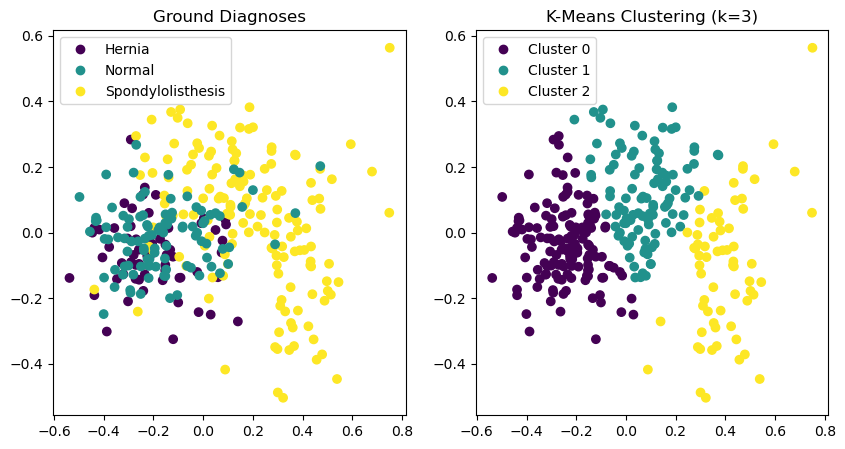
\includegraphics[width=18cm]{./assets/exII3-plot.png}
          \caption{Projected data for the Ground Diagnoses and K-Means Clustering with k=3}
          \label{fig:PartII-ex3}
        \end{figure}

  \item \textbf{Considering the results from questions (1) and (3), identify two ways on how clustering can
          be used to characterize the population of ill and healthy individuals.}

        \vskip 0.3cm
        
        By analyzing our results for exercise 1, we can see that most silhouette scores were moderate,  indicating there is some evidence for clusters to be
         cohesive and well-separated. Additionally, the purity scores were high, raging from 0.63226 until 0.67742, signifying precise clustering in relation to the known categories.
        
        On exercise 3, the visualizations provided a clear comparison between the ground diagnoses and the clustering solution with \(k=3\). This allowed us to visually assess how well
         the clusters align with the actual diagnoses, appearing to perform well.
        
        Given the favorable results obtained in both the quantitative evaluation (silhouette and purity scores) and the visual representations, clustering appears to be a viable method to analyze and categorize individuals based on their health status.
        
        \textbf{Therefore, clustering can be used to characterize the population in ways such as the following:}
        
        \begin{itemize}
            \item \textbf{Identifying High-Risk Groups}: Clustering can group individuals based on certain risk factors for a specific disease, which can help individuals with preventive measures. 
        
            \item \textbf{Identifying Disease Subgroups}: Clustering can be used to identify subgroups within a population of individuals with a particular disease, for example cancer. 
        \end{itemize}

\end{enumerate}
\end{document}
